\begin{figure}[h]
\centering
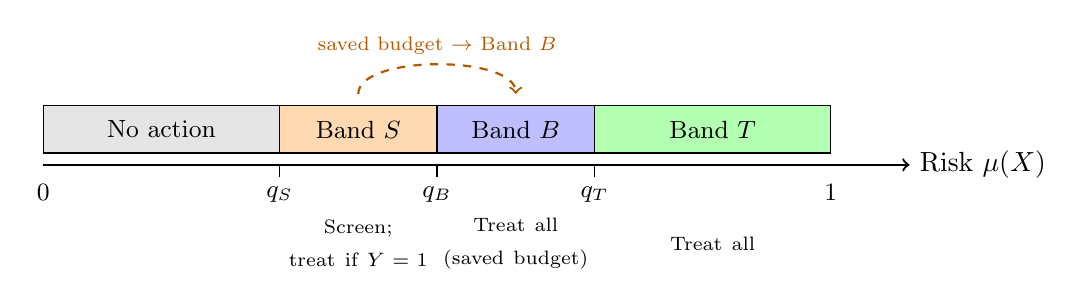
\begin{tikzpicture}[scale=1.0]

    % Risk axis
    \draw[->, thick] (0,0) -- (11,0) node[right] {Risk $\mu(X)$};
    \node at (0,-0.35) {\small $0$};
    \node at (10,-0.35) {\small $1$};

    % Band colours
    % No-treatment zone (grey)
    \fill[gray!20] (0,0.15) rectangle (3,0.75);
    % Band S (yellow)
    \fill[orange!30] (3,0.15) rectangle (5,0.75);
    % Band B (blue, saved budget)
    \fill[blue!25] (5,0.15) rectangle (7,0.75);
    % Band T (green)
    \fill[green!30] (7,0.15) rectangle (10,0.75);

    % Band outlines
    \draw (0,0.15) rectangle (3,0.75);
    \draw (3,0.15) rectangle (5,0.75);
    \draw (5,0.15) rectangle (7,0.75);
    \draw (7,0.15) rectangle (10,0.75);

    % Band labels inside bars
    \node at (1.5,0.45) {\small No action};
    \node at (4.0,0.45) {\small Band $S$};
    \node at (6.0,0.45) {\small Band $B$};
    \node at (8.5,0.45) {\small Band $T$};

    % Quantile tick marks
    \foreach \x/\lbl in {3/$q_S$, 5/$q_B$, 7/$q_T$}{
        \draw (\x, 0) -- (\x, -0.15);
        \node at (\x,-0.38) {\small \lbl};
    }

    % Action labels below bands
    \node[align=center, text width=2cm] at (4.0,-1.0) {\scriptsize Screen;\\ treat if $Y=1$};
    \node[align=center, text width=2.5cm] at (6.0,-1.0) {\scriptsize Treat all\\ (saved budget)};
    \node[align=center, text width=2cm] at (8.5,-1.0) {\scriptsize Treat all};

    % Arrow showing saved budget flow
    \draw[->, dashed, thick, orange!70!black]
        (4.0, 0.9) .. controls (4.0,1.4) and (6.0,1.4) .. (6.0, 0.9)
        node[midway, above] {\scriptsize saved budget $\rightarrow$ Band $B$};

\end{tikzpicture}
\caption{Illustration of the optimal three-band screening strategy. The population is ordered by risk score $\mu(X)$ from left to right. The highest-risk individuals (Band $T$) are treated directly. The middle band (Band $S$) is screened and treated only if $Y=1$, which frees up budget. This saved budget finances Band $B$, an additional treatment band immediately below Band $T$ that would not be reachable without screening.}
\label{fig:illustration}
\end{figure}
